\subsubsection{Impact of Different Types of Program Graphs}
\label{sec:graphs}

\begin{figure}[t]%[thbp]
\begin{center}
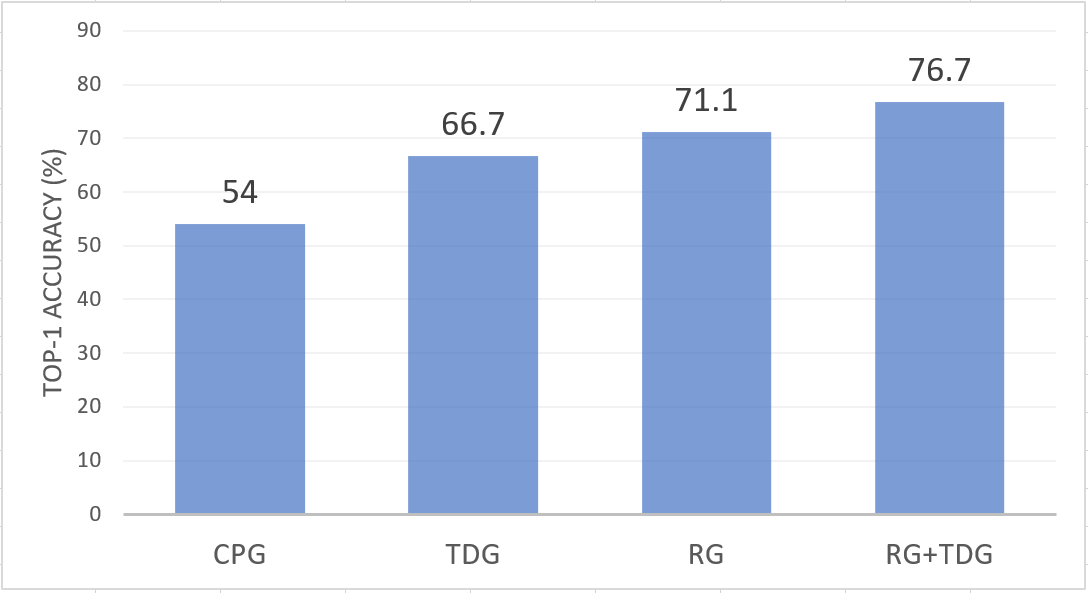
\includegraphics[width=2.3in]{figures/sensi-graphs-name-2}
\vspace{-8pt}
\caption{RQ4. Impact of Input Graphs on Name Prediction}
\label{graph-name-result}
{\bf CPG}: Code Property Graph, {\bf TDG}: Type Dependency Graph, {\bf RG}:Relation Graph. 
\end{center}
\end{figure}



As in any approach, code representation is
important and affects the performance. In this study, we
kept the same neural network architecture, however, changed different
input graphs extracted from source code. In addition to the graphs
used in {\tool} (Relation Graph (RG), Type Dependency Graph (TDG)), we
experimented with code property graph (CPG)~\cite{CPG-2014} since
it has been used in several machine learning approaches for
code~\cite{CPG-2014}. We did not experiment with program dependence
graph (PDG) because it works at the statement level, which does not
help with variable name prediction.

As seen in Figure~\ref{graph-name-result} and
Figure~\ref{graph-type-result}, for variable name prediction, RG helps
the model more than TDG and for variable type prediction, TDG helps
the model more than RG. This is expected because each of them is
designed toward capturing the key features for its problem. For the
dual tasks, the combined graph (RG+TDG) in {\tool} yields the highest
accuracies in both name prediction and type prediction. In contrast,
CPG capturing the dependencies among program elements are not
specifically designed for handling variable names and types, thus, did not
yield high accuracy as TDG, RG, and CG. An interesting observation is
that CPG, which contains lexical, syntax, and dependency information,
did not help the model as much as others. It seems that CPG contains
too much irrelevant information for variable name and type prediction.

\begin{figure}[t]%[thbp]
\begin{center}
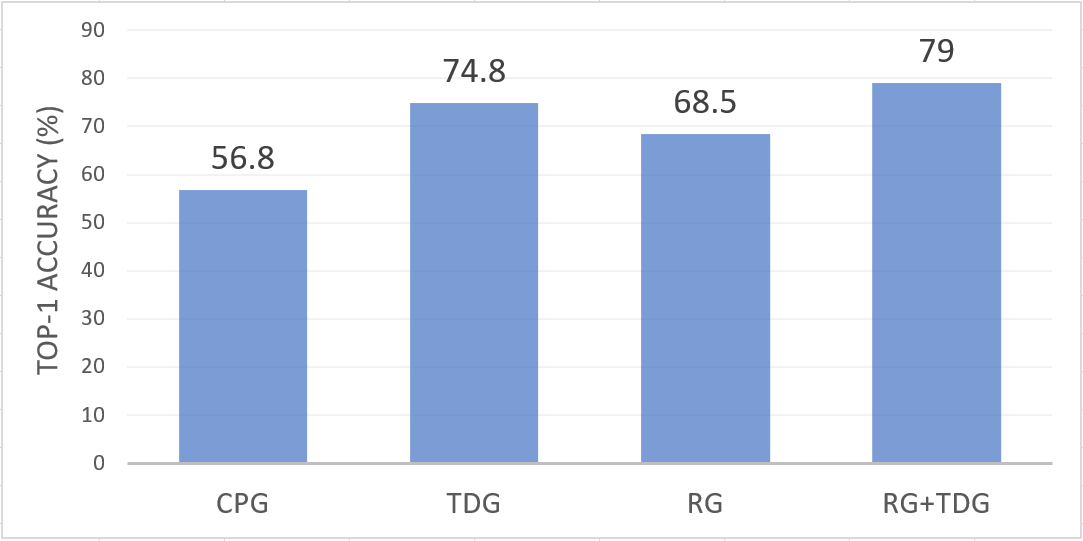
\includegraphics[width=2.3in]{figures/sensi-graphs-type-2}
\vspace{-8pt}
\caption{RQ4. Impact of Input Graphs on Type Prediction}
\label{graph-type-result}
%{\bf CPG}: Code Property Graph, {\bf TDG}: Type Dependency Graph, {\bf RG}:Relation Graph.
\end{center}
\end{figure}

%1. Code property graph is complex but cannot represent the variable relationships and type changes clearly (EEGCN+GCNmf+CPG compared with EEGCN+GCNmf+RG on name prediction; EEGCN+GCNmf+CPG compared with EEGCN+GCNmf+TDG on type prediction)


